\begin{song}{title=\predtitle\centering Kometa \\\large Jaromír Nohavica \vspace*{-0.3cm}}  %% sem se napíše jméno songu a autor

\moveright -1cm \vbox{
\begin{centerjustified}

\begin{varwidth}[t]{0.48\textwidth}\setlength{\parindent}{0.45cm}  %Varianta č. 2 --> Dva sloupce
\sloka 
	^{Ami\z }Spatřil jsem kometu, oblohou letěla,

	chtěl jsem jí zazpívat, ona mi zmizela.

	^{Dmi\z }Zmizela jako ^{G7}laň~u~lesa v remízku,

	^{C}v očích mi zbylo jen ^{E7}pár žlutých

	penízků.

\sloka
	Penízky ukryl jsem do hlíny pod dubem,
	
	až příště přiletí, my už tu nebudem.

	My už tu nebudem, ach, pýcho

	marnivá,

	spatřil jsem kometu, chtěl jsem jí

	zazpívat.
	
\refren
	^{Ami\z}O~vodě, o trávě, ^{Dmi\z }o~lese,
	
	^{G7\z }o~smrti, se kterou smířit ^{C\z }nejde se,
	
	^{Ami\z }o~lásce, o zradě, ^{Dmi\z}o~světě
	
	^{E\z}a~o všech lidech, co kdy ^{E7}žili na téhle
	
	 ^{Ami\z }planetě.
	
\sloka	
	Na hvězdném nádraží cinkají vagóny,
	
	pan Kepler rozepsal nebeské zákony,
	
	hledal, až nalezl v hvězdářských 

	triedrech
	
	tajemství, která teď neseme na 

	bedrech.

\end{varwidth}\mezisloupci\begin{varwidth}[t]{0.5\textwidth}\setlength{\parindent}{0.45cm}
\vspace*{0.375cm}  % V případě varianty č.2 jde odsud text do pravé části
\sloka
	Velká a odvěká tajemství přírody,
	
	že jenom z člověka člověk se narodí,
	
	že kořen s větvemi ve strom se spojuje
	
	a krev našich nadějí vesmírem putuje.

\refren
Na na na\elipsa\dots

\sloka
	Spatřil jsem kometu, byla jak reliéf
	
	zpod rukou umělce, který už nežije,
	
	šplhal jsem do nebe, chtěl jsem ji osahat,
	
	marnost mne vysvlékla celého donaha.
	
\sloka
	Jak socha Davida z bílého mramoru

	stál jsem a hleděl jsem, hleděl jsem

	nahoru.

	Až příště přiletí, ach, pýcho marnivá,

	my už tu nebudem, ale jiný jí zazpívá.


\refren
	O vodě, o trávě, o lese,

	o smrti, se kterou smířit nejde se,

	o lásce, o zradě, o světě,

	bude to písnička o nás a kometě\elipsa\dots



\phantom{.}

\phantom{.}

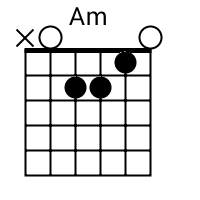
\includegraphics[width = 3cm]{../Akordy/am.png}
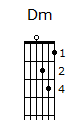
\includegraphics[width = 3cm]{../Akordy/dm.png}

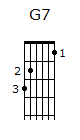
\includegraphics[width = 3cm]{../Akordy/g7.png}
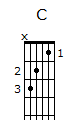
\includegraphics[width = 3cm]{../Akordy/c.png}

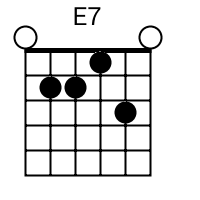
\includegraphics[width = 3cm]{../Akordy/e7.png}

\end{varwidth}

\end{centerjustified}
}
\setcounter{Slokočet}{0}
\end{song}
